\documentclass[../delivery_hospital_report.tex]{subfiles}
\graphicspath{ {images/}{../images/}{../../images/} }

\begin{document}

Um dos maiores problemas nos grandes hospitais da atualidade é a sobrecarga de trabalhos desnecessários, até mesmo fútil, como transporte de medicamentos e exames, para profissionais altamente qualificados. Nos últimos tempos, principalmente por conta do início da Pandemia do COVID19, o número de pessoas que vem frequentando os hospitais é cada vez maior. Em momentos como esses, profissionais da área da saúde perder tempo com serviços automatizáveis corroboram para a ineficiência e demora no atendimento em ambientes hospitalares, que em geral pode custar vidas.

Para contornar esses problemas de automação hospitalar, é cada vez mais comum a utilização de robôs hospitalares, que cumprem a função de realizar trabalhos repetitivos e banais. Isso garante que profissionais da saúde utilizem mais do seu tempo de trabalho exercendo os seus deveres profissionais que fazem sentido com sua profissão. 

Robôs Hospitalares, principalmente graças aos avanços da indústria 4.0, que cumpre funções de automação hospitalar estão cada vez mais em evidência no mercado mundial. Um exemplo disso é robô hospitalar Hospi, que pode ser vista na figura ~\ref{fig: Robô Hospi}, que foi projetado para fazer o transporte de medicamentos por todo um hospital. 


\begin{figure}[h]
\centering
    \caption{Robô Hospi}
    \centering % para centralizarmos a figura
    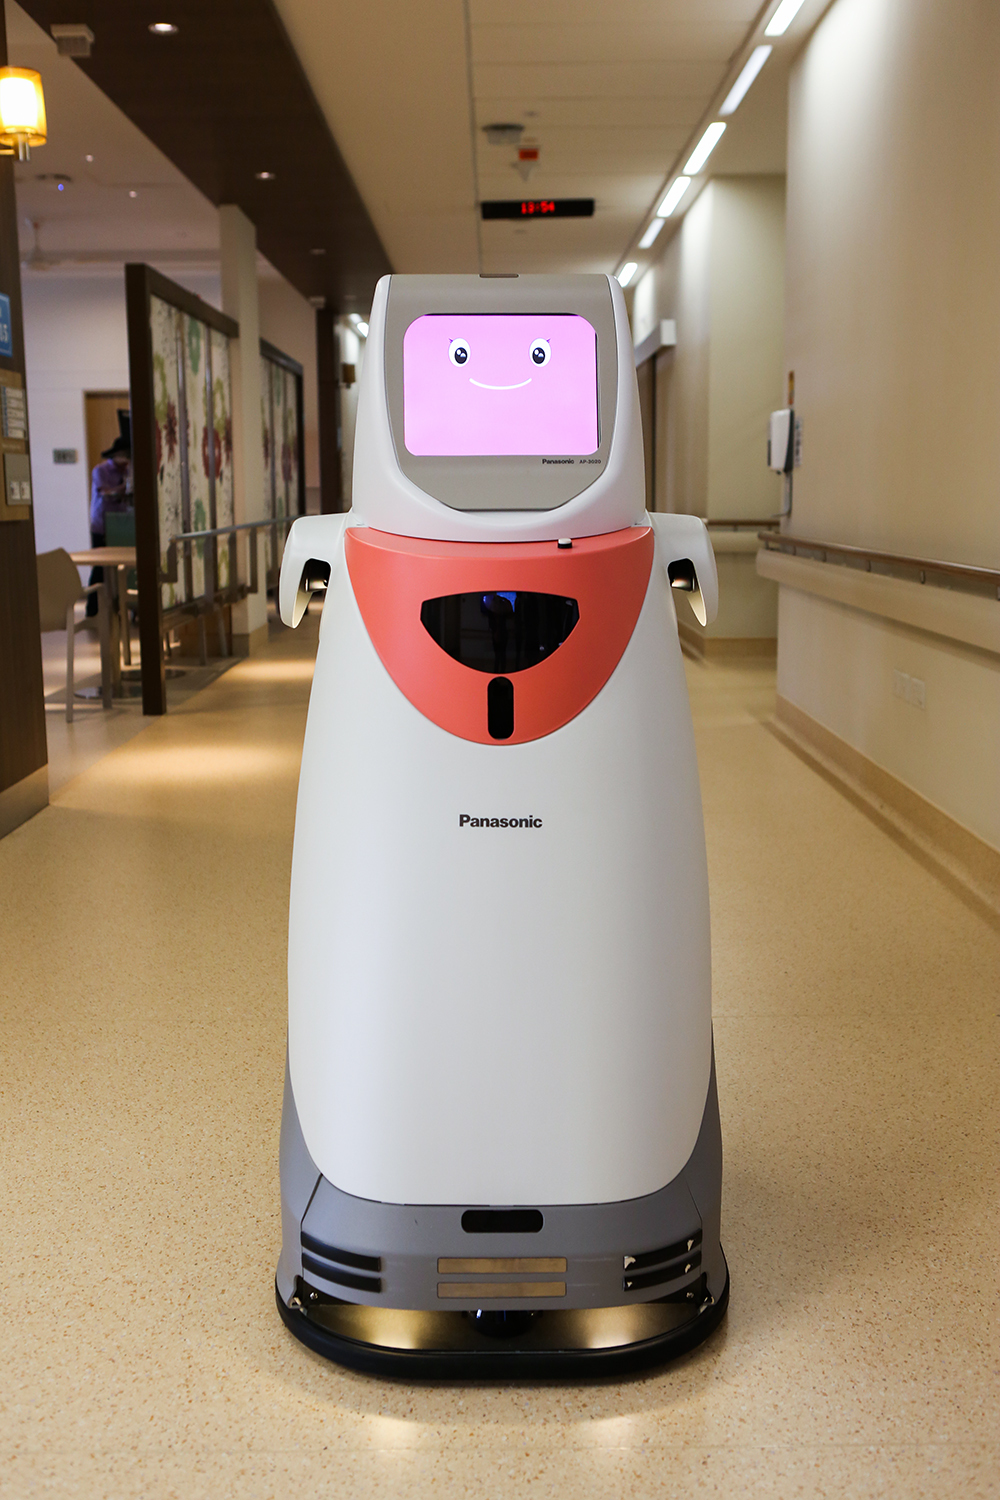
\includegraphics[width=11cm]{hospi.jpg}
    \caption*{Fonte: Business Wire}
    \label{fig: Robô Hospi}
\end{figure}

\end{document}